% DOM, Javascript XML, XSL
% capitolo 7 testo e automa di ciotti
% SLIDE Chiara sui fogli di stile
% Capitolo DOM professional Web Dev e XML processing
%

\documentclass{beamer}
    
    %    \usepackage[english]{babel}
        %\usepackage[latin1]{inputenc}
        %\usepackage[T1]{fontenc}
    
    \mode<presentation>{
      \setbeamertemplate{background canvas}[vertical shading]
      \usetheme{Berkeley}
      \useoutertheme{himinfolines}
    }
      
    \usepackage{ucs}
    \usepackage[utf8]{inputenc}
    \usepackage[english,polutonikogreek,italian,UKenglish,british]{babel}
    \usepackage{graphicx}
    \usepackage{colortbl}
    \usepackage{multicol}
    \usepackage{ulem}
    \usepackage{verbatim}
    \usepackage{alltt}
    \usepackage{ccicons}
    \usepackage{MnSymbol,wasysym}
    \usepackage{tikzsymbols}
    \usepackage{textcomp}
    \usepackage{xmpincl}
    
    \usepackage{parskip}
    \setcounter{nframes}{100}
    \setcounter{nframe}{1}
    \setbeamercovered{dynamic}
    \newenvironment{grcenv}{\begin{otherlanguage}{greek}}{\end{otherlanguage}}
    \newcommand{\g}[1]{\textgreek{#1}}
    \definecolor{darkgreen}{rgb}{0,0.5,0}
    \definecolor{darkblue}{rgb}{0,0,0.5}
    \definecolor{grey}{rgb}{0.5,0.5,0.5}
    \setcounter{tocdepth}{5}
    
    \makeatletter
    
    \makeatother
    %\includexmp{LicencesAndLicensing}
    
    %frame00 metadata
        \title{Codifica TEI - Visualizzazione ed Elaborazione XML}
        \author[A.M. Del Grosso]{Angelo Mario Del Grosso \\ \tiny\textit{..}}
        \institute{\texttt{angelo.delgrosso@ilc.cnr.it} \\\textit{CNR-ILC-LicoLab} \\\url{http://licolab.ilc.cnr.it/}}
        \date{Istituto di Linguistica Computazionale ``A. Zampolli'', \today}
        \AtBeginSection[]{
        \begin{frame}<beamer>
        \addtocounter{nframe}{1}
        \footnotesize
        \frametitle{Progress status}
        \tableofcontents[currentsection,hideothersubsections]
        \end{frame}
        }
    
    \begin{document}
    
    \begin{frame}
        \maketitle
    \end{frame}
    
    \begin{frame}
        \frametitle{Sommario della Lezione}
        \tableofcontents
    \end{frame}
    
    \section{Introduzione}
    
    \begin{frame}
        \frametitle{Visualizzare ed Elaborare documenti XML}
        \addtocounter{nframe}{1}
        
        %\begin{center}
        %    
\includegraphics[width=.2\textwidth]{../imgs/tei-r.pdf}
        %\end{center}
        %\textit{In parte già disponibili nei moduli TEI di base}

         \begin{block}{Perché visualizzare ed elaborare il testo}
        %     \emph{Per la critica testuale indispensabili i moduli}
             \begin{itemize}
                \item Controllare la codifica e correggere i refusi
                \item Assicurarsi che tutto sia stato trascritto correttamente
                \item Mostrare il testo a persone che non conoscono XML-TEI
                \item Disporre di una versione del lavoro fruibile
                \item Manipolare e analizzare le informazioni codificate
            \end{itemize}
         \end{block}
        
    \end{frame}
    
    \begin{frame}
        \frametitle{Visualizzare ed Elaborare documenti XML}
        \addtocounter{nframe}{1}
        
        \begin{block}{I fogli di stile (style sheet)}
           \begin{itemize}
               \item Descrive il modo in cui un documento elettronico deve essere visualizzato
               \item Il mezzo di rendering può variare: lo schermo di un computer, la stampa, i sintetizzatori vocali, ecc.
           \end{itemize}
        \end{block}
        
    \end{frame}

    \begin{frame}
        \frametitle{Visualizzare ed Elaborare documenti XML}
        \addtocounter{nframe}{1}
        
        \begin{block}{Modello del Documento}
           \begin{itemize}
               \item Descrive il modo in cui un documento elettronico deve essere rappresentato e navigato da agenti software
               \item Indipendenza dal linguaggio e dalla piattaforma
           \end{itemize}
        \end{block}
        
    \end{frame}
    
    \begin{frame}
        \frametitle{Visualizzare ed Elaborare documenti XML}
        \addtocounter{nframe}{1}
        
        \begin{block}{Scopo dei fogli di stile}
           \begin{itemize}
               \item \emph{Separazione forma-contenuto}: \textit{la visualizzazione del documento è un processo indipendente (e successivo)}
               \item \emph{Gestione della resa grafica} per molti documenti contemporaneamente: \textit{massima uniformità dello stile}
               \item \emph{Gestione di mezzi diversi} dal monitor: smartphone, sintetizzatore
               vocale, stampante braille, ecc.
           \end{itemize}
        \end{block}
        
    \end{frame}

    \begin{frame}
        \frametitle{Visualizzare ed Elaborare documenti XML}
        \addtocounter{nframe}{1}
        
        \begin{block}{Scopo di un modello per i documenti}
           \begin{itemize}
               \item \emph{Astrazione}: \textit{la navigazione e la elaborazione sono specificate da uno standard e non cambia nelle sue varie implementazioni}
               \item \emph{Uniformità}: \textit{le interfacce sono comuni a tutti i sistemi che implementano il modello}
               \item \emph{Efficacia ed Efficienza}: il modello identifica oggetti, metodi e proprietà utili alla gestione e al controllo programmatico dei documenti. 
           \end{itemize}
        \end{block}
        
    \end{frame}

    \begin{frame}
        \frametitle{Visualizzare ed Elaborare documenti XML}
        \addtocounter{nframe}{1}
        
        \begin{block}{Metodi e Tecnologie}
            \textbf{Quelli più noti e utilizzati sono standard internazionali definiti dal consorzio W3 \url{(http://www.w3.org/Style/CSS)}.}
           \begin{itemize}
            \item XSL: eXtensible Stylesheet Language
            \item DOM: Document Object Model
           \end{itemize}
        \end{block}
        
    \end{frame}

    % \begin{frame}
    %     \frametitle{Modularità della TEI}
    %     \addtocounter{nframe}{1}
        
    %    % \begin{center}
    %     % 
\includegraphics[width=.2\textwidth]{../imgs/tei-r.pdf}
    %     % \end{center}
    
    %     \begin{itemize}
            
    %         \item<1-> parleremo del sistema Modulare della TEI
    %             \begin{itemize}
    %                 \item<1-> Moduli
    %                 \item<1-> Classi
    %                 \item<1-> Macro
    %                 \item<1-> Datatype
    %             \end{itemize} 
    %         \item<2-> parleremo degli elementi basilari
    %             \begin{itemize}
    %                 \item<2-> Intestazione TEI (TEIHeader)
    %                 \item<2-> Elementi e attributi presenti in tutti i documenti TEI
    %                 \item<2-> Esempi di codifica
    %             \end{itemize} 
    %     \end{itemize}
        
    % \end{frame}
    
    \section{XSLT: Documenti Multipli e Versione 2.0}
    \begin{frame}
    \frametitle{Visualizzare ed Elaborare documenti XML}
    \addtocounter{nframe}{1}
    
    %\begin{center}
    %    
\includegraphics[width=.2\textwidth]{../imgs/tei-r.pdf}
    %\end{center}
    %\textit{In parte già disponibili nei moduli TEI di base}

     \begin{block}{XML Slyle Sheet Transformation: Modularità}
        \begin{itemize}
            \item XSLT consente di importare ed includere fogli XSLT dentro altri documenti XSLT
            \item mediante gli elementi \texttt{<xsl:import>} ed \texttt{<xsl:include>} 
        \end{itemize}
     \end{block}

     \begin{block}{XML Slyle Sheet Transformation}
        \begin{itemize}
            \item \textbf{inclusione}: le regole definite nel documento incluso hanno la stessa priorità delle regole definite nel documento XSLT principale.
            \item \textbf{importazione}: le regole definite nel documento principale hanno una priorità maggiore.
        \end{itemize}

     \end{block}


\end{frame}


\begin{frame}
    \frametitle{Visualizzare ed Elaborare documenti XML}
    \addtocounter{nframe}{1}
    
    \textbf{Dichiarazione XSD dell'elemento xsl:include}

    \begin{center}
        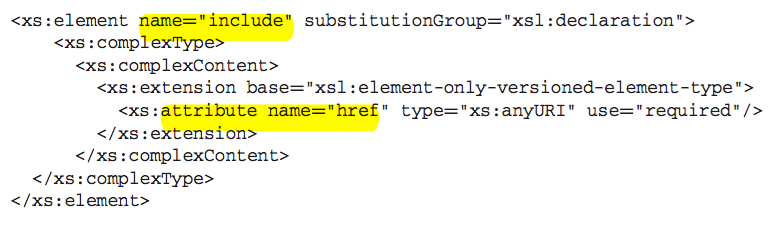
\includegraphics[width=.8\textwidth]{imgs/elementXSL-Include.png}
    \end{center}

\end{frame}

\begin{frame}
    \frametitle{Visualizzare ed Elaborare documenti XML}
    \addtocounter{nframe}{1}
    
    %\begin{center}
    %    
\includegraphics[width=.2\textwidth]{../imgs/tei-r.pdf}
    %\end{center}
    %\textit{In parte già disponibili nei moduli TEI di base}

     \begin{block}{XML Slyle Sheet Transformation: xsl:include}
        Dato un foglio esterno \texttt{esterno.xsl} per includerlo nel foglio principale si impiega l'elemento: \texttt{<xsl:include href="esterno.xsl"/>}
     \end{block}

\end{frame}

\begin{frame}
    \frametitle{Visualizzare ed Elaborare documenti XML}
    \addtocounter{nframe}{1}
    
    \textbf{Dichiarazione XSD dell'elemento xsl:import}

    \begin{center}
        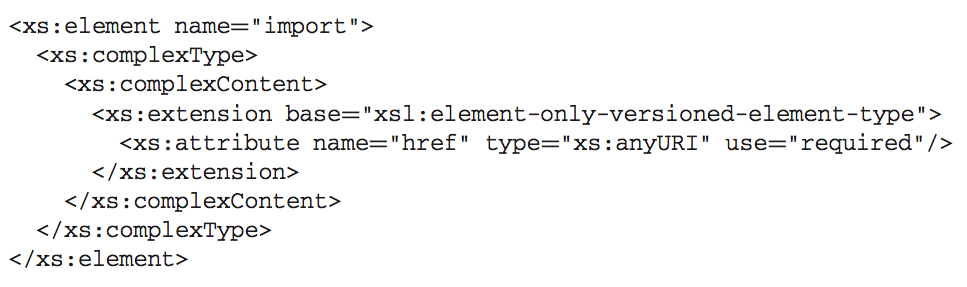
\includegraphics[width=.8\textwidth]{imgs/elementXSL-Import.png}
    \end{center}

\end{frame}

\begin{frame}
    \frametitle{Visualizzare ed Elaborare documenti XML}
    \addtocounter{nframe}{1}
    
    %\begin{center}
    %    
\includegraphics[width=.2\textwidth]{../imgs/tei-r.pdf}
    %\end{center}
    %\textit{In parte già disponibili nei moduli TEI di base}

     \begin{block}{XML Slyle Sheet Transformation: xsl:import}
        \texttt{<xsl:import href="esterno.xsl"/>}
        \\\texttt{<xsl:template match="/" >}
        \\\texttt{ <xsl:apply-imports/>}
        \\\texttt{</xsl:template>}
     \end{block}

\end{frame}

\begin{frame}
    \frametitle{Visualizzare ed Elaborare documenti XML}
    \addtocounter{nframe}{1}
    
    %\begin{center}
    %    
\includegraphics[width=.2\textwidth]{../imgs/tei-r.pdf}
    %\end{center}
    %\textit{In parte già disponibili nei moduli TEI di base}

     \begin{block}{XML Slyle Sheet Transformation: documenti multipli}
        \begin{itemize}
            \item Accedere ai nodi di un documento XML esterno a quello che si sta elaborando
            \item Utilizzando la funzionalità \texttt{document()}
        \end{itemize}

     \end{block}

     \begin{block}{XML Slyle Sheet Transformation: documenti multipli}
        \texttt{<xsl:value-of}
        \\\texttt{ select="document(’altro.xml’)/TEI/text/@type"}
        \\\texttt{/>}

     \end{block}

\end{frame}

\begin{frame}
    \frametitle{Visualizzare ed Elaborare documenti XML}
    \addtocounter{nframe}{1}
    
    %\begin{center}
    %    
\includegraphics[width=.2\textwidth]{../imgs/tei-r.pdf}
    %\end{center}
    %\textit{In parte già disponibili nei moduli TEI di base}

     \begin{block}{XML Slyle Sheet Transformation: XSLT 2.0}
        La \textit{recommendation} W3C per XSLT 2.0 è stata pubblicata nel 2007
     \end{block}

     \begin{block}{XML Slyle Sheet Transformation: documenti multipli}
       
        \texttt{<xsl:stylesheet} 
            \\\texttt{xmlns:xsl="http://www.w3.org/1999/XSL/Transform"} 
            \\\texttt{version="2.0" >}


     \end{block}

\end{frame}


\begin{frame}
    \frametitle{Visualizzare ed Elaborare documenti XML}
    \addtocounter{nframe}{1}
    
    %\begin{center}
    %    
\includegraphics[width=.2\textwidth]{../imgs/tei-r.pdf}
    %\end{center}
    %\textit{In parte già disponibili nei moduli TEI di base}

     \begin{block}{XML Slyle Sheet Transformation: XSLT 2.0}
        XSLT 2.0 che permette di creare un documento di output (xml, html, xhtml, text).
     \end{block}

     \begin{block}{XML Slyle Sheet Transformation: documenti multipli}
       
        \texttt{<xsl:template match="/" >}
        \\\texttt{ <xsl:result-document method="html" href="output.html" >}
        \\\texttt{ <xsl:apply-templates/>}
        \\\texttt{ </xsl:result-document>}
        \\\texttt{</xsl:template>}
            
     \end{block}

\end{frame}

\begin{frame}
    \frametitle{Visualizzare ed Elaborare documenti XML}
    \addtocounter{nframe}{1}
    
    %\begin{center}
    %    
\includegraphics[width=.2\textwidth]{../imgs/tei-r.pdf}
    %\end{center}
    %\textit{In parte già disponibili nei moduli TEI di base}

     \begin{block}{XML Slyle Sheet Transformation: XSLT 2.0}
        XSLT 2.0 che permette di creare anche documenti multipli.
     \end{block}

     \begin{block}{XML Slyle Sheet Transformation: XSLT 2.0 esempio}
        \texttt{<template match="//div/[@type='book']" >}
        \\\texttt{<xsl:for-each select="div/[@type='chapter']" >}
        \\\texttt{<xsl:result-document}
           \\\texttt{method="html"}
           \\\texttt{href="{@n}.html" >}
           \\\texttt{<xsl:apply-templates/>}
        \\\texttt{</xsl:result-document>}
        \\\texttt{</xsl:for-each>}
        \\\texttt{</xsl:template>}
    
    \end{block}

\end{frame}

\begin{frame}
    \frametitle{Visualizzare ed Elaborare documenti XML}
    \addtocounter{nframe}{1}
    
    %\begin{center}
    %    
\includegraphics[width=.2\textwidth]{../imgs/tei-r.pdf}
    %\end{center}
    %\textit{In parte già disponibili nei moduli TEI di base}

     \begin{block}{XML Slyle Sheet Transformation: XSLT 2.0}
        \begin{itemize}
            \item elemento \texttt{<xsl:for-each-group>}: permette di selezionare un set di items
            \item processare un gruppo per volta
        \end{itemize}
        
     \end{block}

     \begin{block}{XML Slyle Sheet Transformation: XSLT 2.0}
        \textit{Possibili attributi}
        \begin{itemize}
            \item group-by
            \item group-adjacent
            \item group-starting-with
            \item group-ending-with
        \end{itemize}
    
    \end{block}

\end{frame}

\begin{frame}
    \frametitle{Visualizzare ed Elaborare documenti XML}
    \addtocounter{nframe}{1}
    
        \textit{Esempio elemento for-each-group}

    \begin{center}
        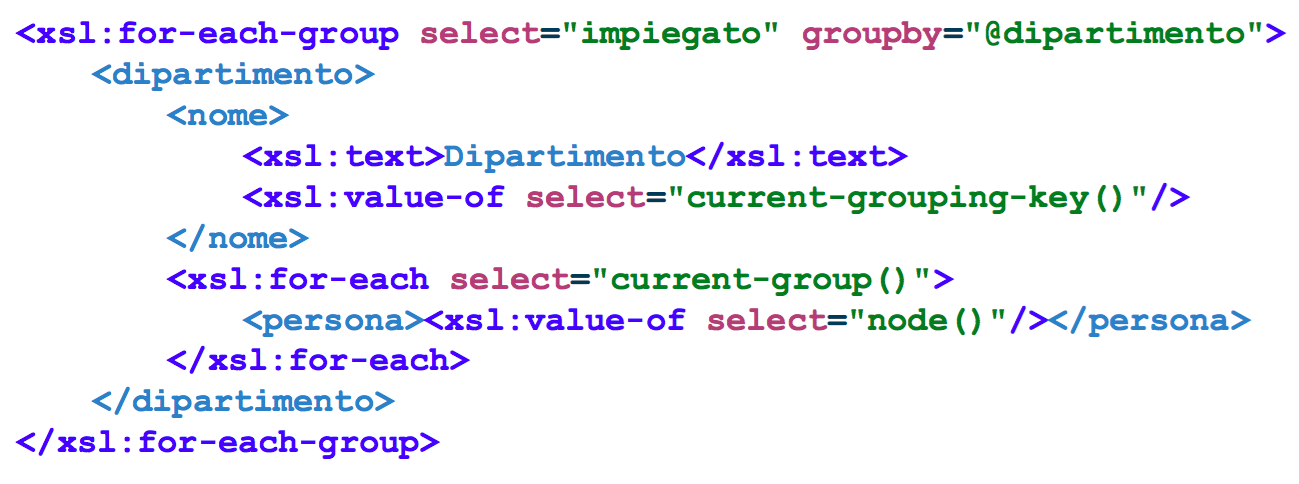
\includegraphics[width=.8\textwidth]{imgs/esempio-groupBy.png}
    \end{center}

\end{frame}

\begin{frame}
    \frametitle{Visualizzare ed Elaborare documenti XML}
    \addtocounter{nframe}{1}
    
        \textit{Espressioni condizionali if()}

    \begin{center}
        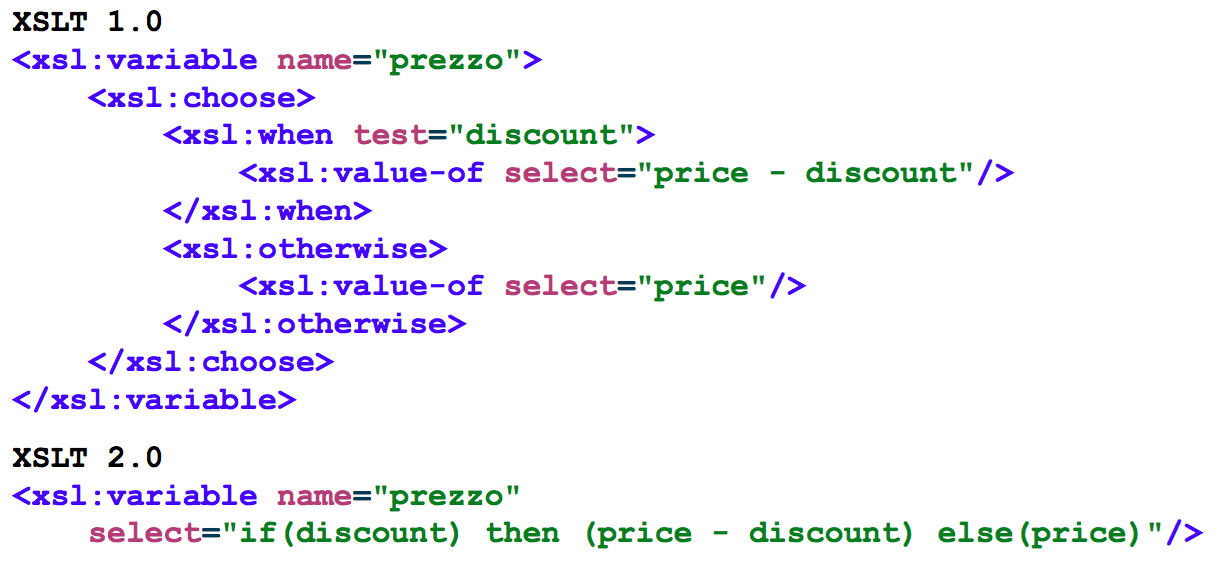
\includegraphics[width=.8\textwidth]{imgs/esempio-espressioneCondizionale.png}
    \end{center}

\end{frame}




    
    \section{XML Transformations: Un esempio con XML-TEI}
    \begin{frame}
    \frametitle{Visualizzare ed Elaborare documenti XML}
    \addtocounter{nframe}{1}
    
        \textit{tutti i nomi di elementi TEI devono essere preceduti dal
        prefisso \textbf{tei:}}

    \begin{center}
        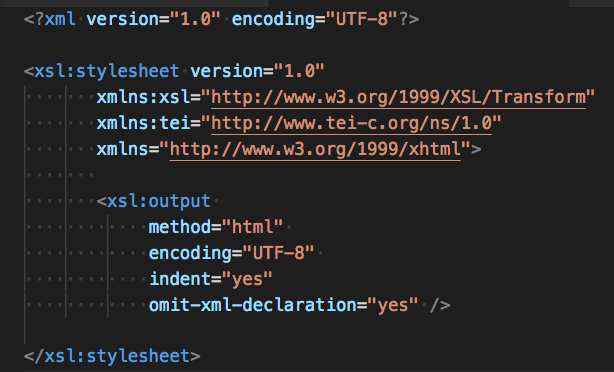
\includegraphics[width=.8\textwidth]{imgs/EsempioCommentato1.png}
    \end{center}

\end{frame}


\begin{frame}
    \frametitle{Visualizzare ed Elaborare documenti XML}
    \addtocounter{nframe}{1}
    
        \textit{creare lo “scheletro” del documento finale, nel nostro caso un HTML}

    \begin{center}
        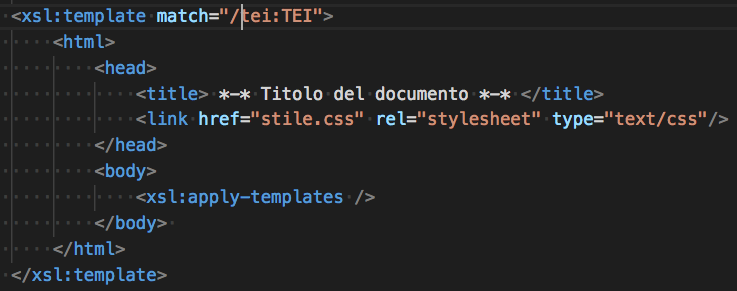
\includegraphics[width=.8\textwidth]{imgs/EsempioCommentato2.png}
    \end{center}

\end{frame}

\begin{frame}
    \frametitle{Visualizzare ed Elaborare documenti XML}
    \addtocounter{nframe}{1}
    
        \textit{definire ad esempio una regola per l’intestazione TEI (\texttt{<teiHeader>})}

    \begin{center}
        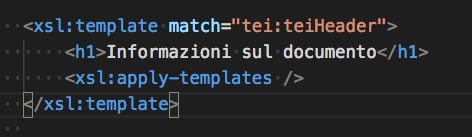
\includegraphics[width=.8\textwidth]{imgs/EsempioCommentato3.png}
    \end{center}

\end{frame}


\begin{frame}
    \frametitle{Visualizzare ed Elaborare documenti XML}
    \addtocounter{nframe}{1}
    
        \textit{Componenti dell'elemento \textbf{tei:text}}

    \begin{center}
        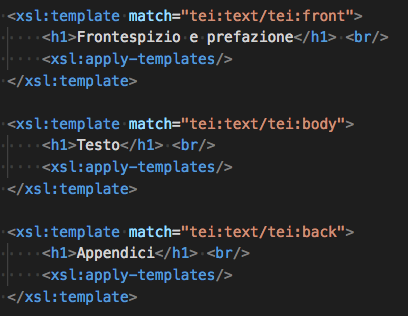
\includegraphics[width=.8\textwidth]{imgs/EsempioCommentato4.png}
    \end{center}

\end{frame}

\begin{frame}
    \frametitle{Visualizzare ed Elaborare documenti XML}
    \addtocounter{nframe}{1}
    
        \textit{Divisioni del testo}

    \begin{center}
        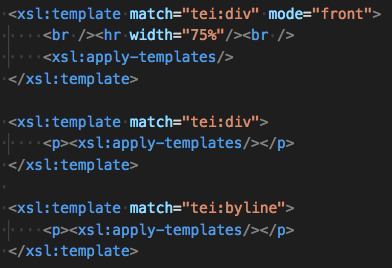
\includegraphics[width=.8\textwidth]{imgs/EsempioCommentato5.png}
    \end{center}

\end{frame}


\begin{frame}
    \frametitle{Visualizzare ed Elaborare documenti XML}
    \addtocounter{nframe}{1}
    
        \textit{Per la poesia}

    \begin{center}
        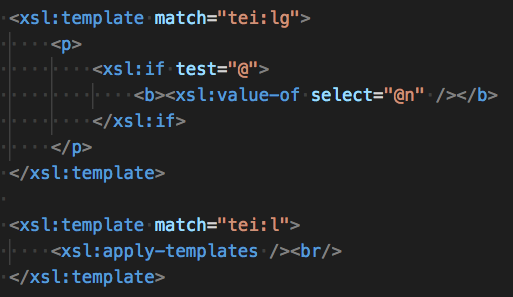
\includegraphics[width=.8\textwidth]{imgs/EsempioCommentato6.png}
    \end{center}

\end{frame}


\begin{frame}
    \frametitle{Visualizzare ed Elaborare documenti XML}
    \addtocounter{nframe}{1}
    
        \textit{Elementi Phrase-Level}

    \begin{center}
        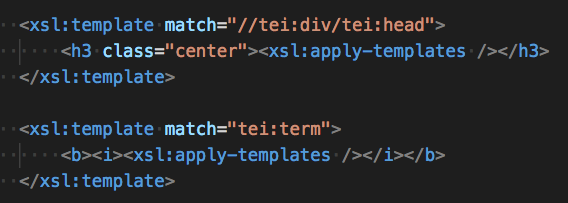
\includegraphics[width=.8\textwidth]{imgs/EsempioCommentato7.png}
    \end{center}

\end{frame}


\begin{frame}
    \frametitle{Visualizzare ed Elaborare documenti XML}
    \addtocounter{nframe}{1}
    
        \textit{Interventi Editoriali}

    \begin{center}
        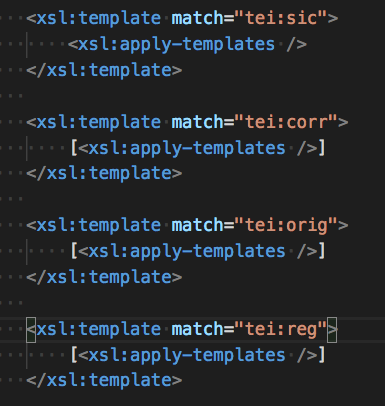
\includegraphics[width=.8\textwidth]{imgs/EsempioCommentato8.png}
    \end{center}

\end{frame}

\begin{frame}
    \frametitle{Visualizzare ed Elaborare documenti XML}
    \addtocounter{nframe}{1}
    
        \textit{Altri elementi}

    \begin{center}
        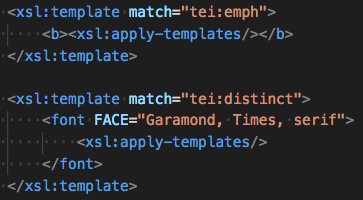
\includegraphics[width=.8\textwidth]{imgs/EsempioCommentato9.png}
    \end{center}

\end{frame}

\begin{frame}
    \frametitle{Visualizzare ed Elaborare documenti XML}
    \addtocounter{nframe}{1}
    
        \textit{Elemento \texttt{<hi>} distinto in base all'attributo \texttt{@rend}}

    \begin{center}
        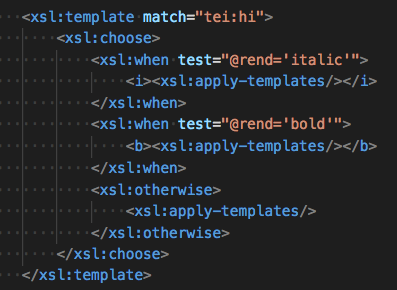
\includegraphics[width=.8\textwidth]{imgs/EsempioCommentato10.png}
    \end{center}

\end{frame}

\begin{frame}
    \frametitle{Visualizzare ed Elaborare documenti XML}
    \addtocounter{nframe}{1}
    
        \textit{Elementi vuoti e milestone}

    \begin{center}
        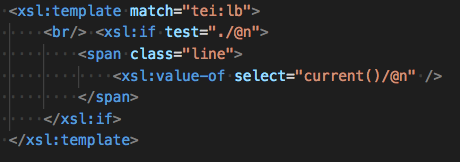
\includegraphics[width=.8\textwidth]{imgs/EsempioCommentato11.png}
    \end{center}

\end{frame}





    
    \section{Panoramica sul Document Object Model (DOM)}
    % The Document Object Model
% The document object model (DOM) is, as previously mentioned, a way of representing the document
% independent of browser type. It allows a developer to access the document via a common set of objects,
% properties, methods, and events, and to alter the contents of the web page dynamically using scripts.
% You should be aware that some small variations are usually added to the DOM by the browser
% vendor. So, to guarantee that you don’t fall afoul of a particular implementation, the W3C has
% provided a generic set of objects, properties, and methods that should be available in all browsers, in
% the form of the DOM standard.
% The DOM Standard
% We haven’t talked about the DOM standard so far, and for a particular reason: It’s not the easiest
% standard to follow. Supporting a generic set of properties and methods has proved to be a very
% complex task, and the DOM standard has been broken down into separate levels and sections
% to deal with the different areas. The different levels of the standard are all at differing stages of
% completion.

% Level 0
% Level 0 is a bit of a misnomer, because there wasn’t really a level 0 of the standard. This term in fact
% refers to the “old way” of doing things—the methods implemented by the browser vendors before the
% DOM standard. Someone mentioning level 0 properties is referring to a more linear notation of accessing
% properties and methods. For example, typically you’d reference items on a form with the following code:
% document.forms[0].elements[1].value = "button1";
% We’re not going to cover such properties and methods in this chapter, because they have been
% superseded by newer methods.

% Level 1
% Level 1 is the first version of the standard. It is split into two sections: One is defined as core
% (objects, properties, and methods that can apply to both XML and HTML) and the other as HTMLThe Document Object Model
% ❘ 235
% (HTML‐specific objects, properties, and methods). The first section deals with how to go about
% navigating and manipulating the structure of the document. The objects, properties, and methods in
% this section are very abstract. The second section deals with HTML only and offers a set of objects
% corresponding to all the HTML elements. This chapter mainly deals with the second section—
% level 1 of the standard.
% In 2000, level 1 was revamped and corrected, though it only made it to a working draft and not to a
% full W3C recommendation.

% Level 2
% Level 2 is complete and many of the properties, methods, and events have been implemented
% by today’s browsers. It has sections that add specifications for events and style sheets to the
% specifications for core and HTML‐specific properties and events. (It also provides sections on
% views and traversal ranges, neither of which is covered in this book; you can find more information
% at www.w3.org/TR/2000/PR‐DOM‐Level‐2‐Views‐20000927/ and www.w3.org/TR/2000/
% PR‐DOM‐Level‐2‐Traversal‐Range‐20000927/ .)

% Level 3
% Level 3 achieved recommendation status in 2004. It is intended to resolve a lot of the complications
% that still exist in the event model in level 2 of the standard, and adds support for XML features,
% such as content models and being able to save the DOM as an XML document.
% Level 4
% In May 2014, DOM level 4 reached candidate recommendation status. It consolidates DOM level 3
% with several independent components. At the time of this writing, no modern browser supports
% DOM level 4, although that will change in the future.
    
    \section{XML DOM Programming API: Un esempio TEI}
    \begin{frame}
    \frametitle{Visualizzare ed Elaborare documenti XML}
    \addtocounter{nframe}{1}
    
    %\begin{center}
    %    
\includegraphics[width=.2\textwidth]{../imgs/tei-r.pdf}
    %\end{center}
    %\textit{In parte già disponibili nei moduli TEI di base}

     \begin{block}{Documenti Object Model (DOM): Esercizio}
       Caricare il file testTeiNS.xml con javascript e manipolarlo con DOM e Xpath per costruire una visualizzazione appropriata
     \end{block}

     \begin{block}{Documenti Object Model (DOM)}
        Scrivere un foglio di stile e applicarlo con javascript al documento DOM caricando il file testTeiNS.xml
     \end{block}


\end{frame}
    
    \end{document}